\section{Auswertung}
\label{sec:Auswertung}
Die Schallgeschwindigkeiten in Wasser und Acryl sind durch
\begin{align*}
  c_{\symup{Acryl}} &= 2730\,\unit{\meter\per\second}\\
  c_{\symup{Wasser}}  &= 1480\,\unit{\meter\per\second}
\end{align*}
gegeben \cite{schallgeschwindigkeit}.

\subsection{Maße des Acrylbocks}
Die Messung ergibt für die Länge $l$ und Höhe $h$ des Acrylblocks.
\begin{align*}
  \symup{l} &= 15,028\,\unit{\centi\meter}\\
  \symup{h} &= 8,025\,\unit{\centi\meter}.
\end{align*}
Die Messwerte für die Lage und Größe der Löcher sind in \autoref{tab:Abstand_Durchmesser} zu finden.
\begin{table}
  \centering
  \begin{tabular}{c c c}
    \toprule
    Störstelle & $\symup{s}/\unit{\centi\meter}$ & $\symup{d}/\unit{\centi\meter}$\\
    \midrule
    $\symup{1}  $ & $6,180$ & $0,145$ \\
    $\symup{2}  $ & $6,060$ & $0,145$ \\
    $\symup{3}  $ & $1,505$ & $0,565$ \\
    $\symup{4}  $ & $2,385$ & $0,490$ \\
    $\symup{5}  $ & $3,220$ & $0,400$ \\
    $\symup{6}  $ & $3,980$ & $0,385$ \\
    $\symup{7}  $ & $4,880$ & $0,300$ \\
    $\symup{8}  $ & $5,595$ & $0,260$ \\
    $\symup{9}  $ & $6,390$ & $0,290$ \\
    $\symup{10} $ & $7,210$ & $0,270$ \\
    $\symup{11} $ & $1,945$ & $0,975$ \\
    \bottomrule
  \end{tabular}
  \caption{Abstand und Durchmesser der Löcher von der unteren Kante aus gemessen.}
  \label{tab:Abstand_Durchmesser}
\end{table}
Die Messwerte können zum Abgleich mit den Ergebnissen der Ultraschallmessung verwendet werden.

\subsection{Messung der Schallgeschwindigkeit in Acryl}
\label{sec:SchallgeschwindigkeitAcryl}
Die Laufzeiten $\symup{t}_{\symup{A}}$, die mit dem A-Scan bestimmt worden sind, sind für die Störstellen in
\autoref{tab:Laufzeiten} zu finden.
\begin{table}
  \centering
  \begin{tabular}{c c}
    \toprule
    Störstelle & $\symup{t}_{\symup{A}}/\unit{\micro\second}$ \\
    \midrule
    11 & 41,6 \\
     4 & 40,5 \\
     5 & 34,9 \\
     6 & 29,4 \\
     7 & 24,1 \\
     8 & 18,2 \\
     9 & 12,0 \\
    \bottomrule
  \end{tabular}
  \caption{Laufzeiten der Störstellen.}
  \label{tab:Laufzeiten}
\end{table}
In \autoref{fig:Laufzeiten} werden die Laufzeiten gegen die Höhe des Acrylblocks abzüglich der Abstände zu den
Störstellen aufgetragen. \autoref{eqn:Strecke} lässt sich zu einer linearen Regressionsformel umformen. Bei der
die Anpassungsschichtdicke $d$ als Ordinate bestimmt wird.
\begin{equation*}
  2h = c\cdot t + d
\end{equation*} 
Aus der linearen Regression ergeben sich die Werte
\begin{align*}
  c &= (2944 \pm 99)\,\unit{\meter\per\second} \\
  b &= (-3 \pm 3)\cdot 10^{-3}\,\unit{\meter}\,. \\
\end{align*}

\begin{figure}
  \centering
  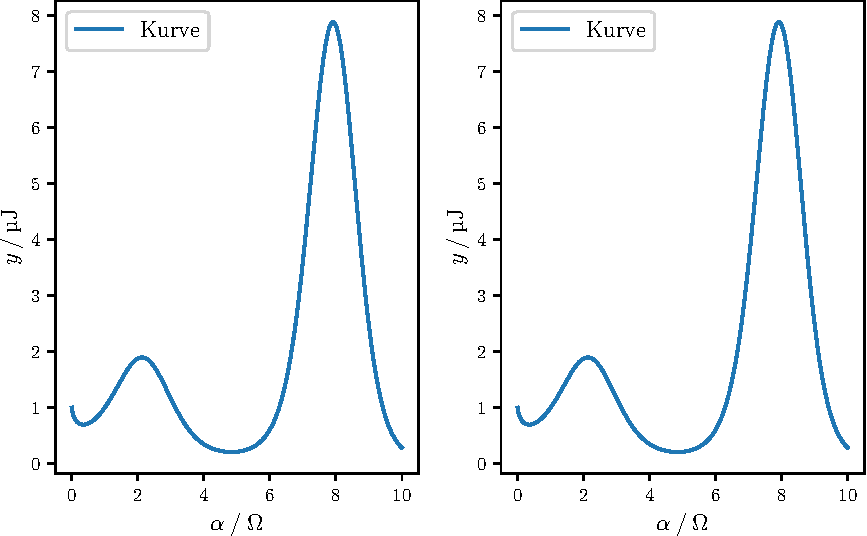
\includegraphics{plot.pdf}
  \caption{Laufzeiten in Abhängigkeit der Höhe des Acrylblocks abzüglich der Abstände zu den Störstellen und
  lineare Regression.}
  \label{fig:Laufzeiten}
\end{figure}

\subsection{Tiefe der der Störstellen}
\label{sec:Tiefe}
Die Laufzeiten bis zu den Störstellen sind in \autoref{tab:Laufzeit_oben_unten} zu finden.
\begin{table}
  \centering
  \begin{tabular}{c c c }
    \toprule
    Störstelle & $\symup{t}_{\symup{Unten}}/\unit{\micro\second}$ & $\symup{t}_{\symup{Oben}}/\unit{\micro\second}$\\
    \midrule
     1 & 14,1 & 48,8 \\
     2 & 15,3 & 44,6 \\
     3 & 49,9 & 10,8 \\
     4 & 40,5 & 17,2 \\
     5 & 34,9 & 23,3 \\
     6 & 29,4 & 29,5 \\
     7 & 24,1 & 35,4 \\
     8 & 18,2 & 41,1 \\
     9 & 12,0 & 46,9 \\
    10 &  6,2 & 53,0 \\
    11 & 41,6 & 12,6 \\
    \bottomrule
  \end{tabular}
  \caption{Laufzeiten bis zu den Störstellen von beiden Seiten gemessen.}
  \label{tab:Laufzeit_oben_unten}
\end{table}
Es wurde eine Laufzeitkorrektur von $\symup{t}_{\symup{Korrektur}} = 1,6\,\unit{\micro\second}$ bestimmt.
Aus \autoref{eqn:Strecke} kann die Strecke bis zur Störstelle berechnet werden. Aus den bestimmten Werte lassen sich
die Dicken der Störstellen bestimmen. Die Abstände und Dicken der Störstellen sind in \autoref{tab:Abstand} zu finden.
\begin{table}
  \centering
  \begin{tabular}{c c c c}
    \toprule
    Störstellen & $\symup{s}_{\symup{Unten}}/\unit{\centi\meter}$ & $\symup{s}_{\symup{Oben}}/\unit{\centi\meter}$ & $\symup{d}/\unit{\centi\meter}$ \\
    \midrule
     1 & 1,706 & 6,443 & 0,124 \\
     2 & 1,870 & 5,869 & 0,285 \\
     3 & 6,593 & 1,256 & 0,176 \\
     4 & 5,310 & 2,129 & 0,586 \\
     5 & 4,545 & 2,962 & 0,518 \\
     6 & 3,795 & 3,808 & 0,422 \\
     7 & 3,071 & 4,614 & 0,340 \\
     8 & 2,266 & 5,392 & 0,367 \\
     9 & 1,420 & 6,183 & 0,422 \\
    10 & 0,628 & 7,016 & 0,381 \\
    11 & 5,460 & 1,501 & 1,064 \\
    \bottomrule
  \end{tabular}
  \caption{Abstände zu den Störstellen und Dicke der Störstellen.}
  \label{tab:Abstand}
\end{table}

\subsection{Auflösungsvermögen}
\label{sec:Aufloesungvermoegen}
Das Auflösungsvermögen wurden an den Störstellen 1 und 2 mit einer $1\,\unit{\mega\hertz}$- und einer
$2\,\unit{\mega\hertz}$-Sonde überprüft. Die Ergebnisse sind in \autoref{fig:aufloesung1}  und in
\autoref{fig:aufloesung2} zu sehen.
\begin{figure}
    \centering
    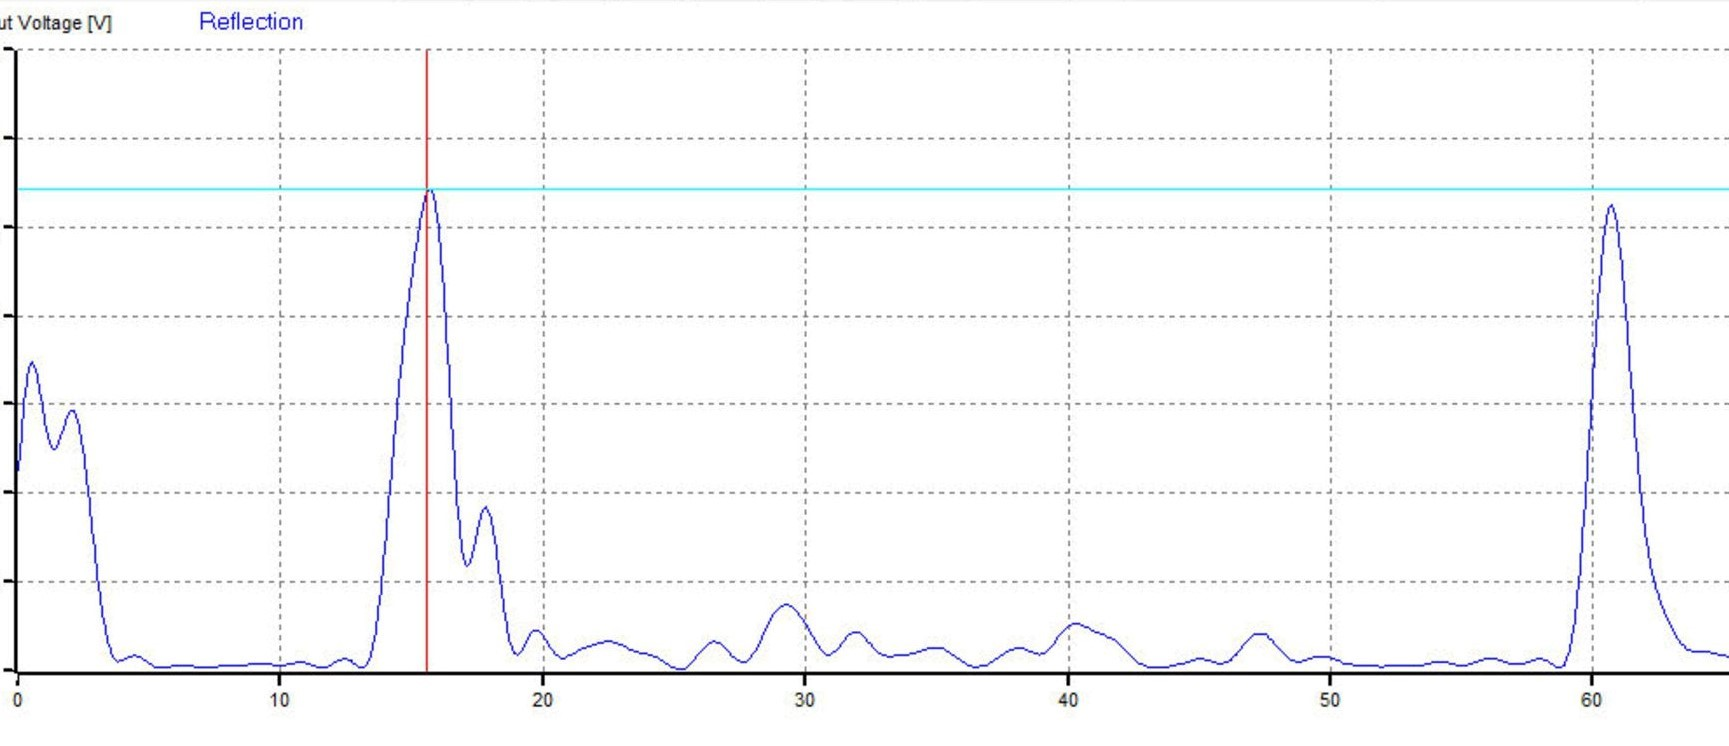
\includegraphics{messwerte/UntersuchungAufloesungsvermoegen/1MhzNo1.jpg}
    \caption{A-Scan der Störstellen mit einer $1\,\unit{\mega\hertz}$-Sonde.}
    \label{fig:aufloesung1}
\end{figure}

\begin{figure}
  \centering
  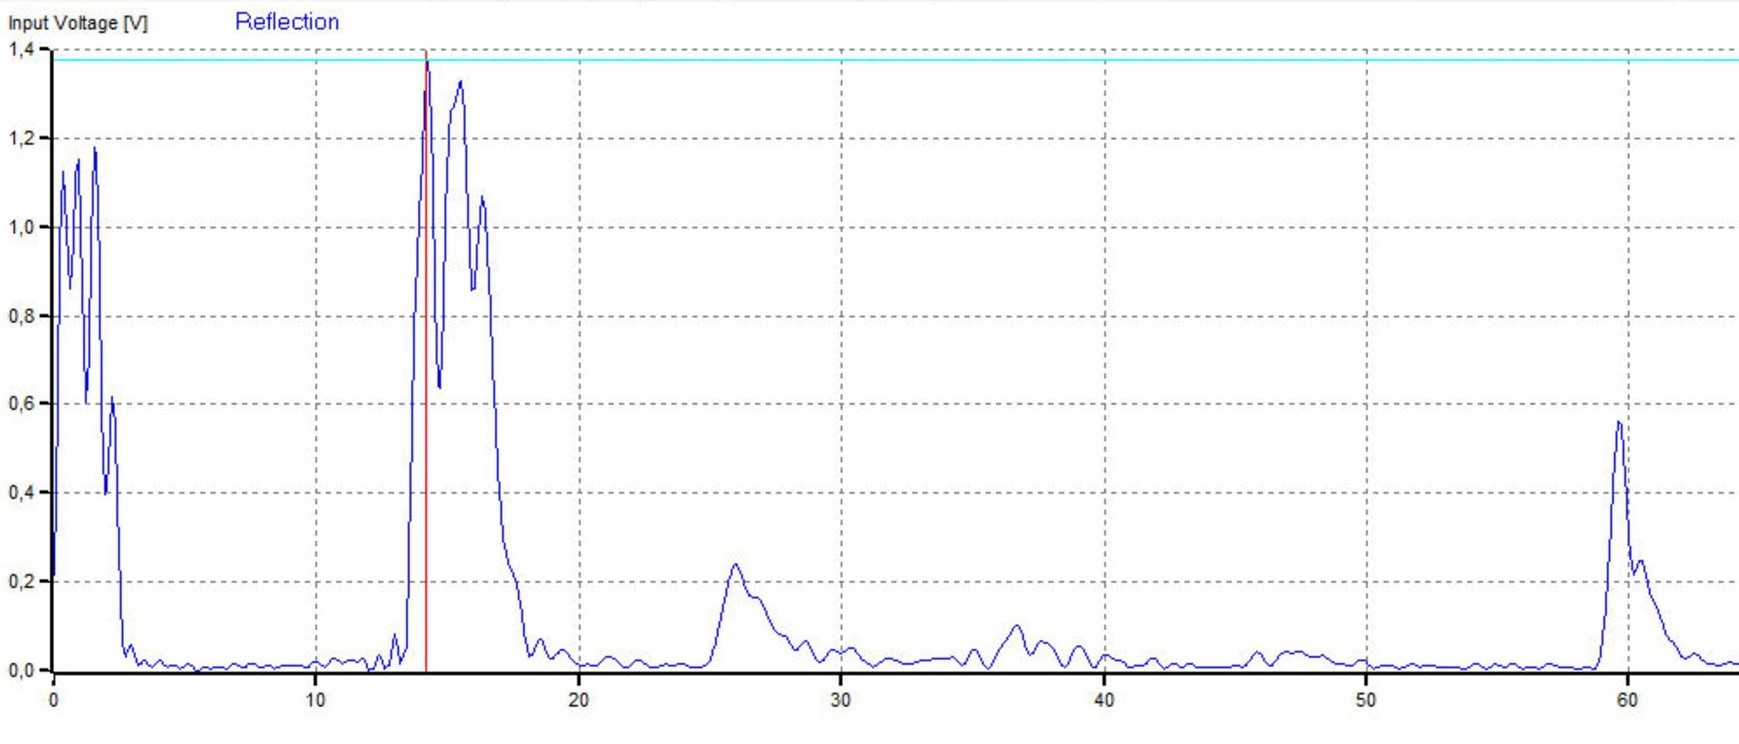
\includegraphics{messwerte/UntersuchungAufloesungsvermoegen/2MhzNo1.jpg}
  \caption{A-Scan der Störstellen mit einer $2\,\unit{\mega\hertz}$-Sonde.}
  \label{fig:aufloesung2}
\end{figure}
Insgesamt fällt auf, dass die $2\,\unit{\mega\hertz}$-Sonde ein höheres Auflösungsvermögen
als die $1\,\unit{\mega\hertz}$-Sonde hat. Im Gegensatz dazu fällt die Amplitude der $2\,\unit{\mega\hertz}$
Messung schneller ab.

\subsection{B-Scan eines Acrylblocks}
Die B-Scans der Acrylblocks mit einer $2\,\unit{\mega\hertz}$-Sonde sind in \autoref{fig:Acryl1} und
\autoref{fig:Acryl2} abgebildet.
\begin{figure}
  \centering
  \includegraphics[width=0.7\textwidth]{messwerte/BScanAcrylBlock/2Mhz.jpg}
  \caption{B-Scan des Acrylblocks.}
  \label{fig:Acryl1}
\end{figure}

\begin{figure}
  \centering
  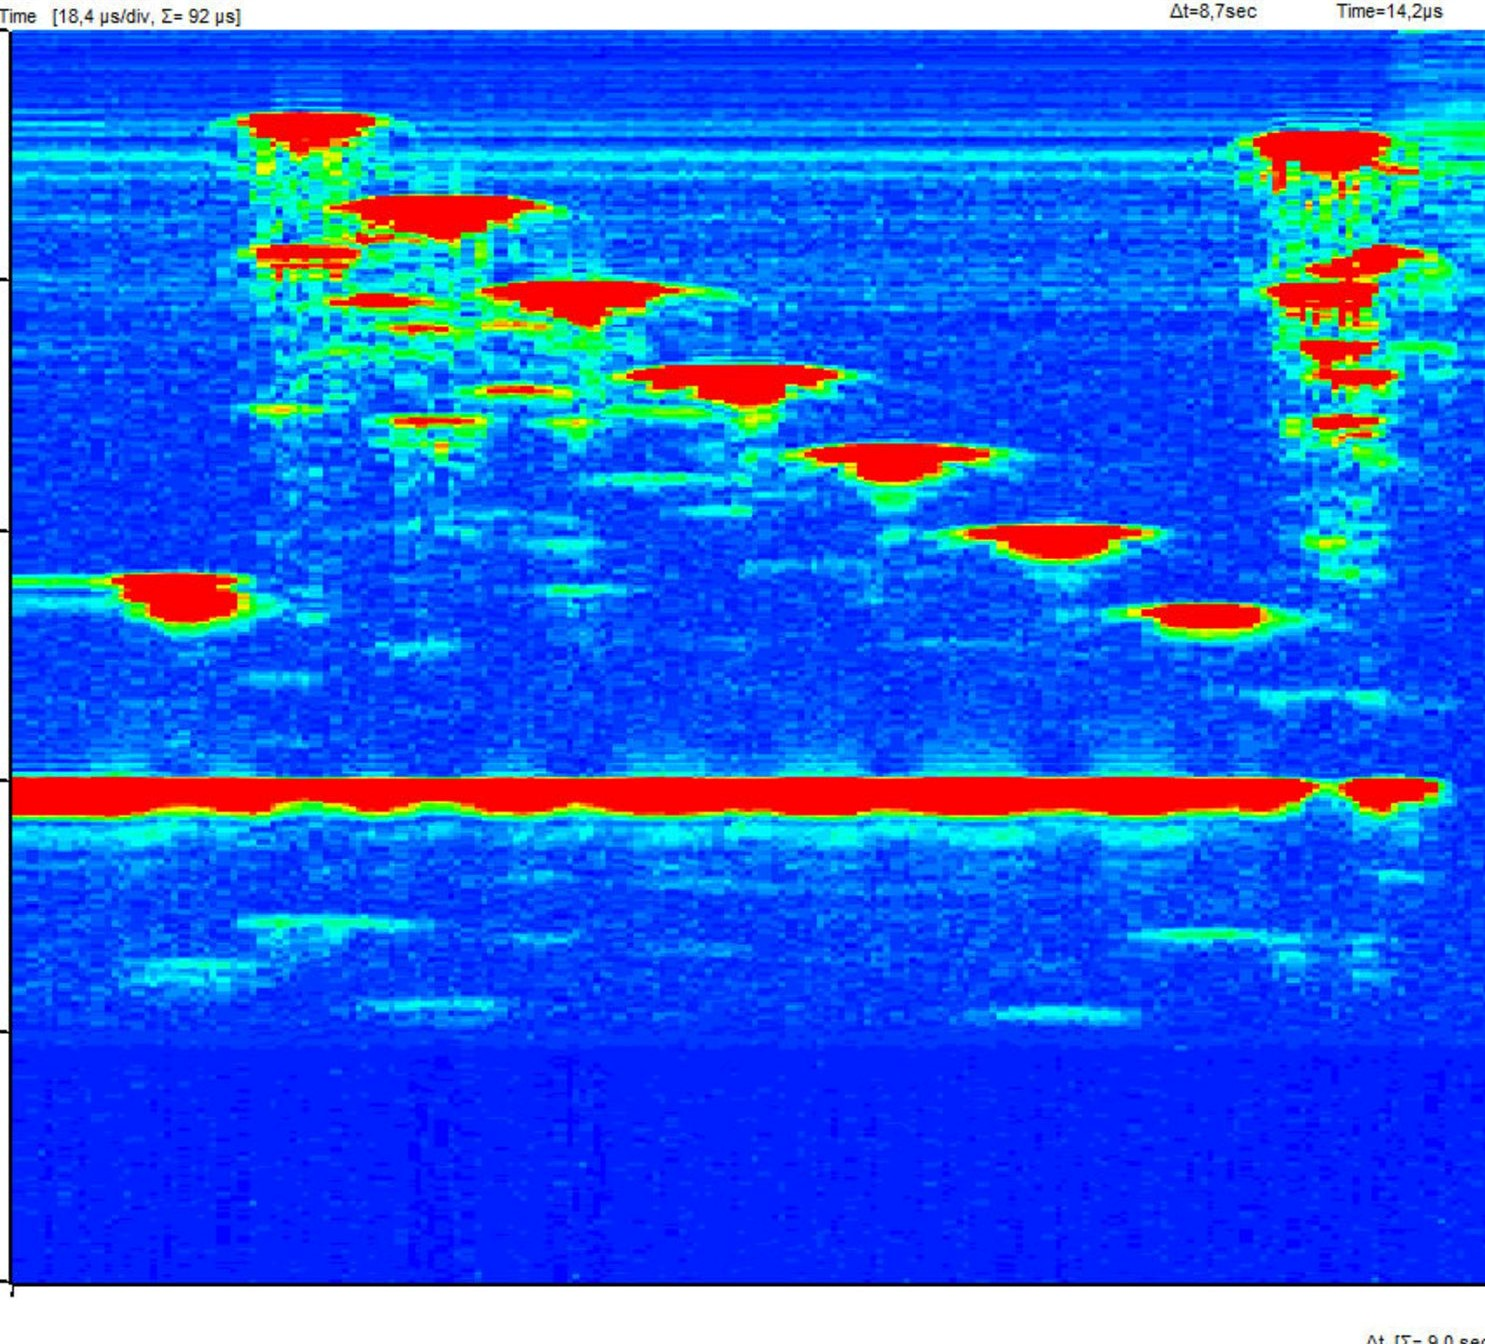
\includegraphics[width=0.7\textwidth]{messwerte/BScanAcrylBlock/umgedreht.jpg}
  \caption{B-Scan des Acrylblocks anders herum gemessen.}
  \label{fig:Acryl2}
\end{figure}
Die Laufzeiten der Störstellen lassen sich aus den B-Scans bestimmen. Mit Hilfe von \autoref{eqn:Strecke} lassen
sich die Störstellen und anschließend die Dicken bestimmen. Die ermittelten Werte sind in \autoref{tab:BScanDicke}
dargestellt.
\begin{table}
  \centering
  \begin{tabular}{c c c c c c}
    \toprule
    Störstellen & $t_{\symup{unten}}/\unit{\micro\second}$ & $t_{\symup{oben}}/\unit{\micro\second}$ & $s_{\symup{unten}}/\unit{\centi\meter}$ & $s_{\symup{oben}}/\unit{\centi\meter}$ & $d/\unit{\centi\meter}$ \\
    \midrule
     1 & 12 & 42 & 1,4 & 5,5 & 0,109 \\
     2 & 14 & 43 & 1,7 & 5,7 & 0,068 \\
     3 & 45 &  8 & 5,9 & 0,9 & 0,123 \\
     4 & 40 & 16 & 5,2 & 2,0 & 0,082 \\
     5 & 32 & 20 & 4,1 & 2,5 & 0,136 \\
     6 & 25 & 27 & 3,2 & 3,5 & 0,136 \\
     7 & 20 & 38 & 2,5 & 5,0 & 0,054 \\
     8 & 16 & 40 & 2,0 & 5,2 & 0,082 \\
     9 & 12 & 42 & 1,4 & 5,5 & 0,109 \\
    10 &  5 & 55 & 0,5 & 7,3 & 0,027 \\
    11 & 40 &  7 & 5,2 & 0,7 & 0,205 \\
    \bottomrule
  \end{tabular}
  \caption{Laufzeiten, Abstände und Dicken der Störstellen mit dem B-Scan ermittelt.}
  \label{tab:BScanDicke}
\end{table}

\subsection{B-Scan eines Brustmodels}
Durch Ertasten lassen sich zwei Tumore feststellen. Ein kleiner direkt über der Brustwarze und ein größerer rechts
unten in der Brust. Diese finden sich auch im B-Scan der Brust wieder. Die B-Scans sind in \autoref{fig:klein} und
\autoref{fig:gross} dargestellt.
\begin{figure}
  \centering
  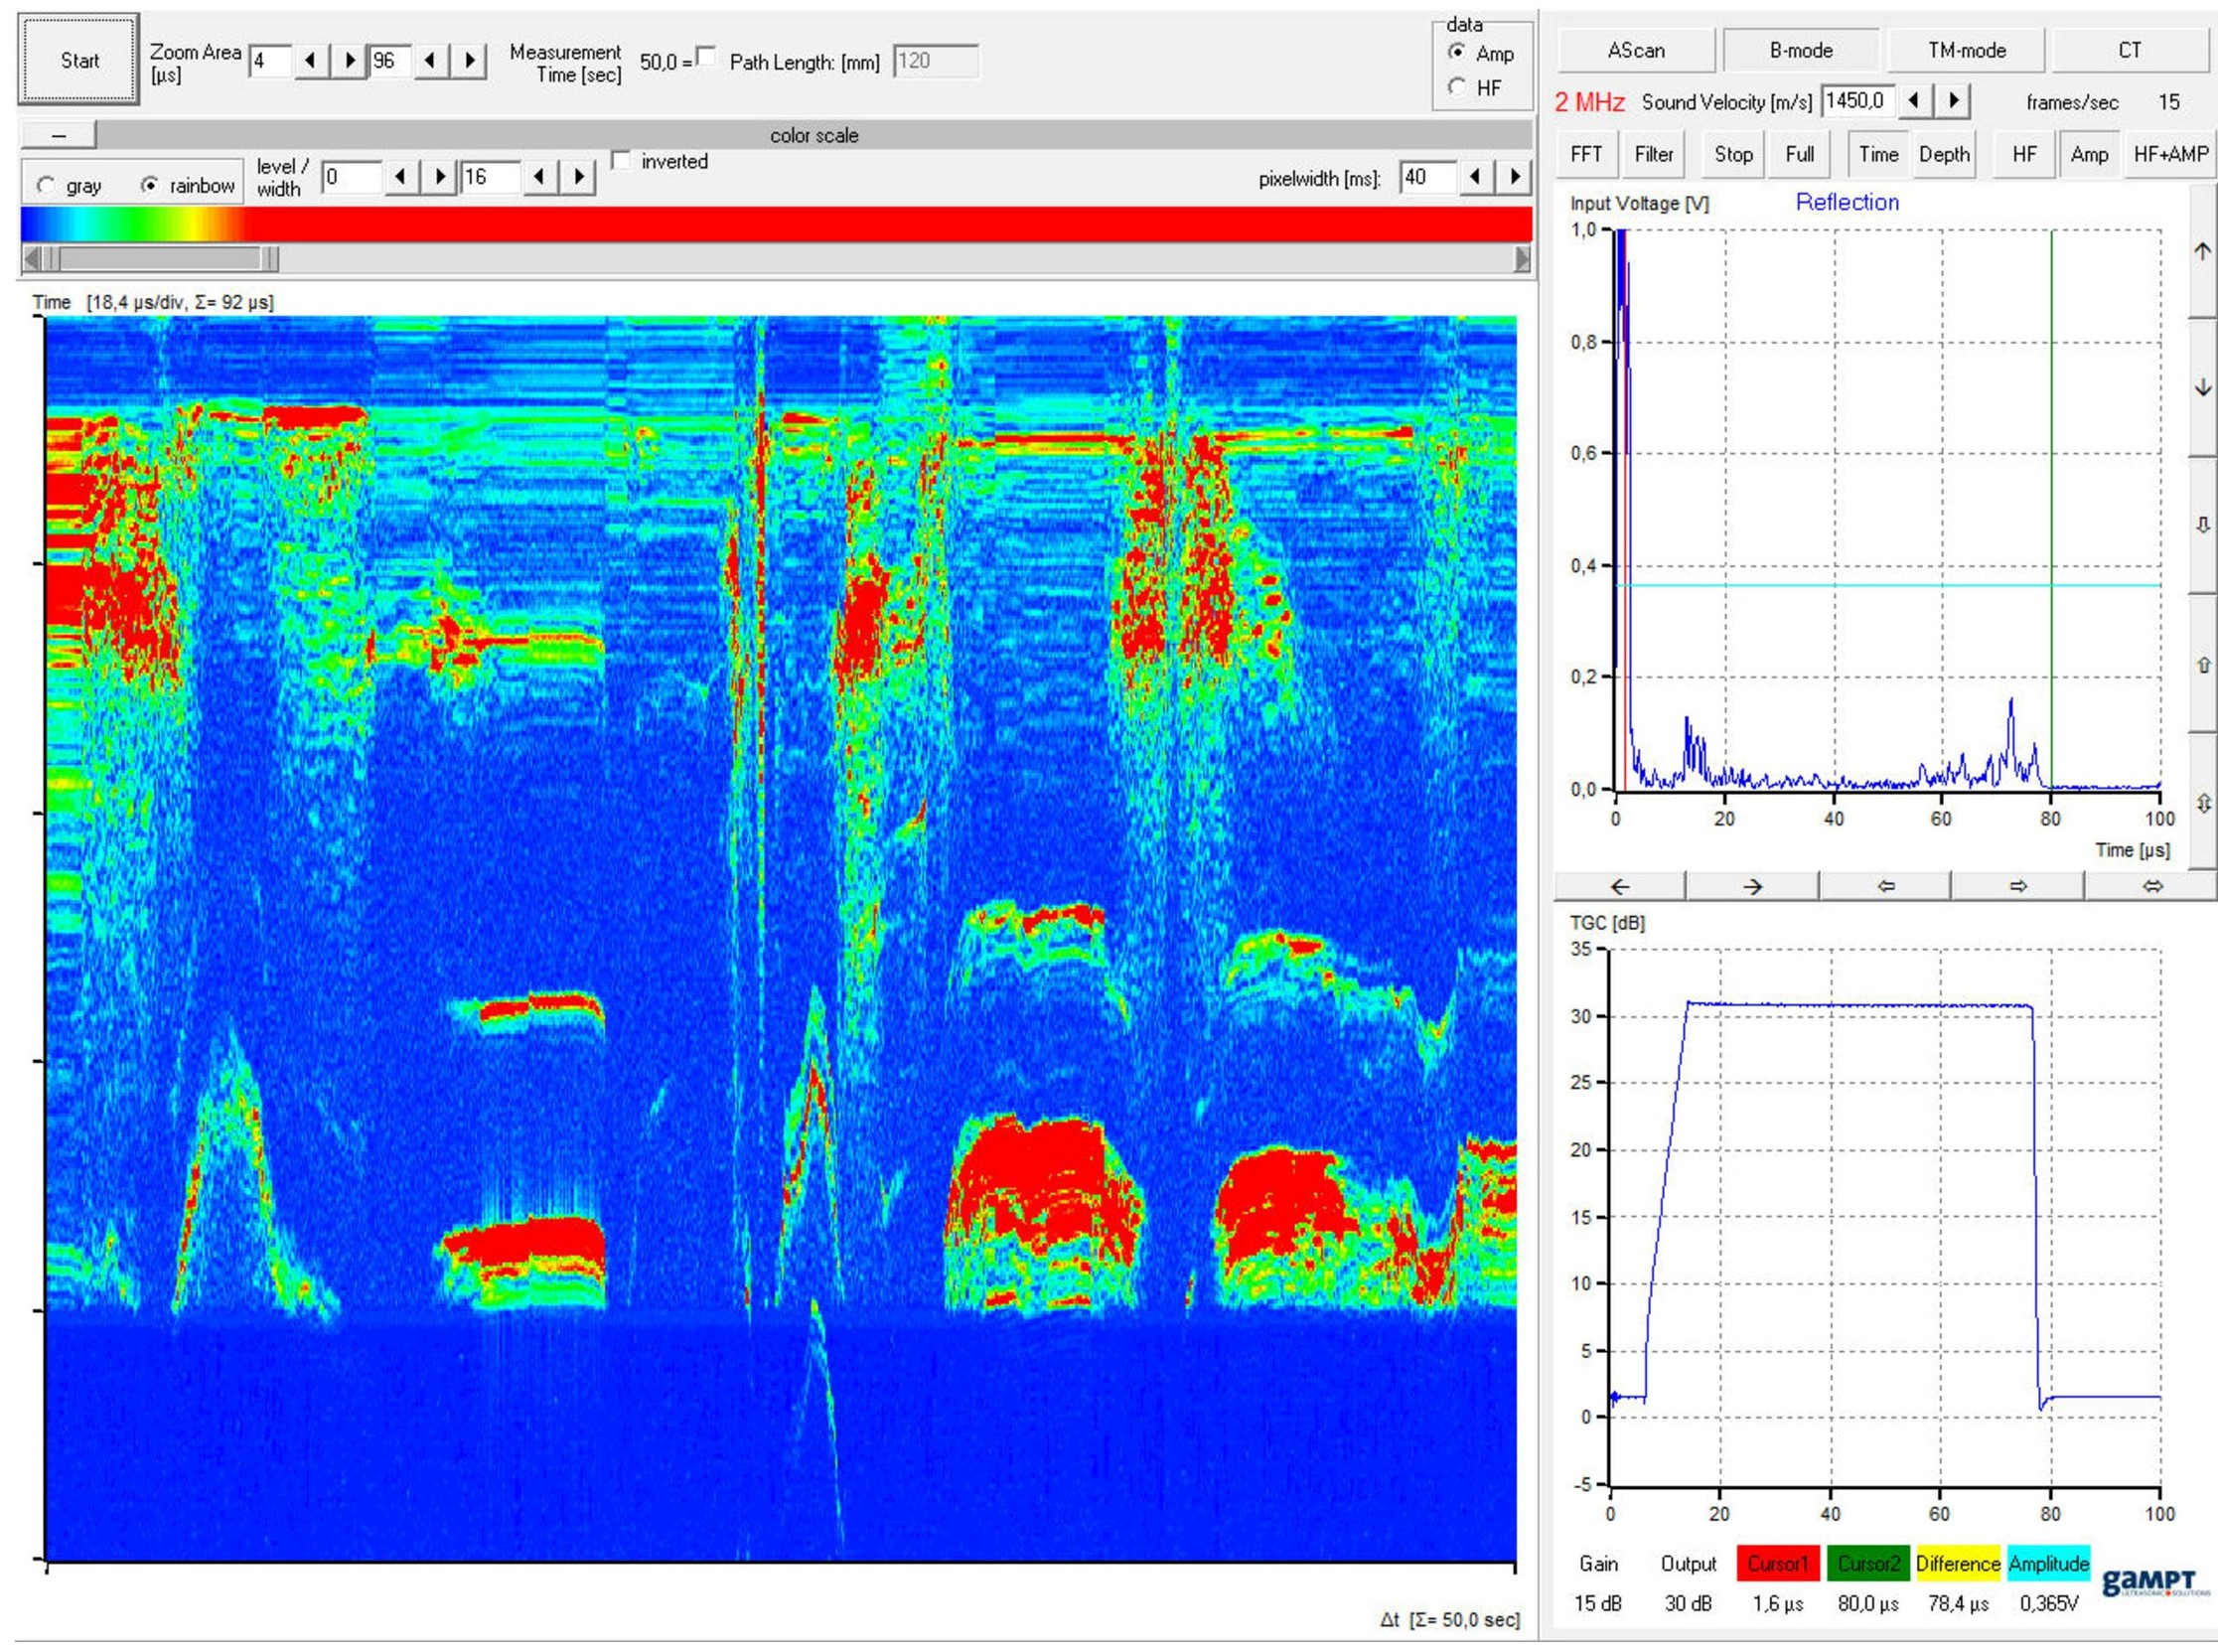
\includegraphics[width=\textwidth]{messwerte/Boobie/Obenklein.jpg}
  \caption{B-Scan des kleineren Tumors über der Brustwarze.}
  \label{fig:klein}
\end{figure}
\begin{figure}
  \centering
  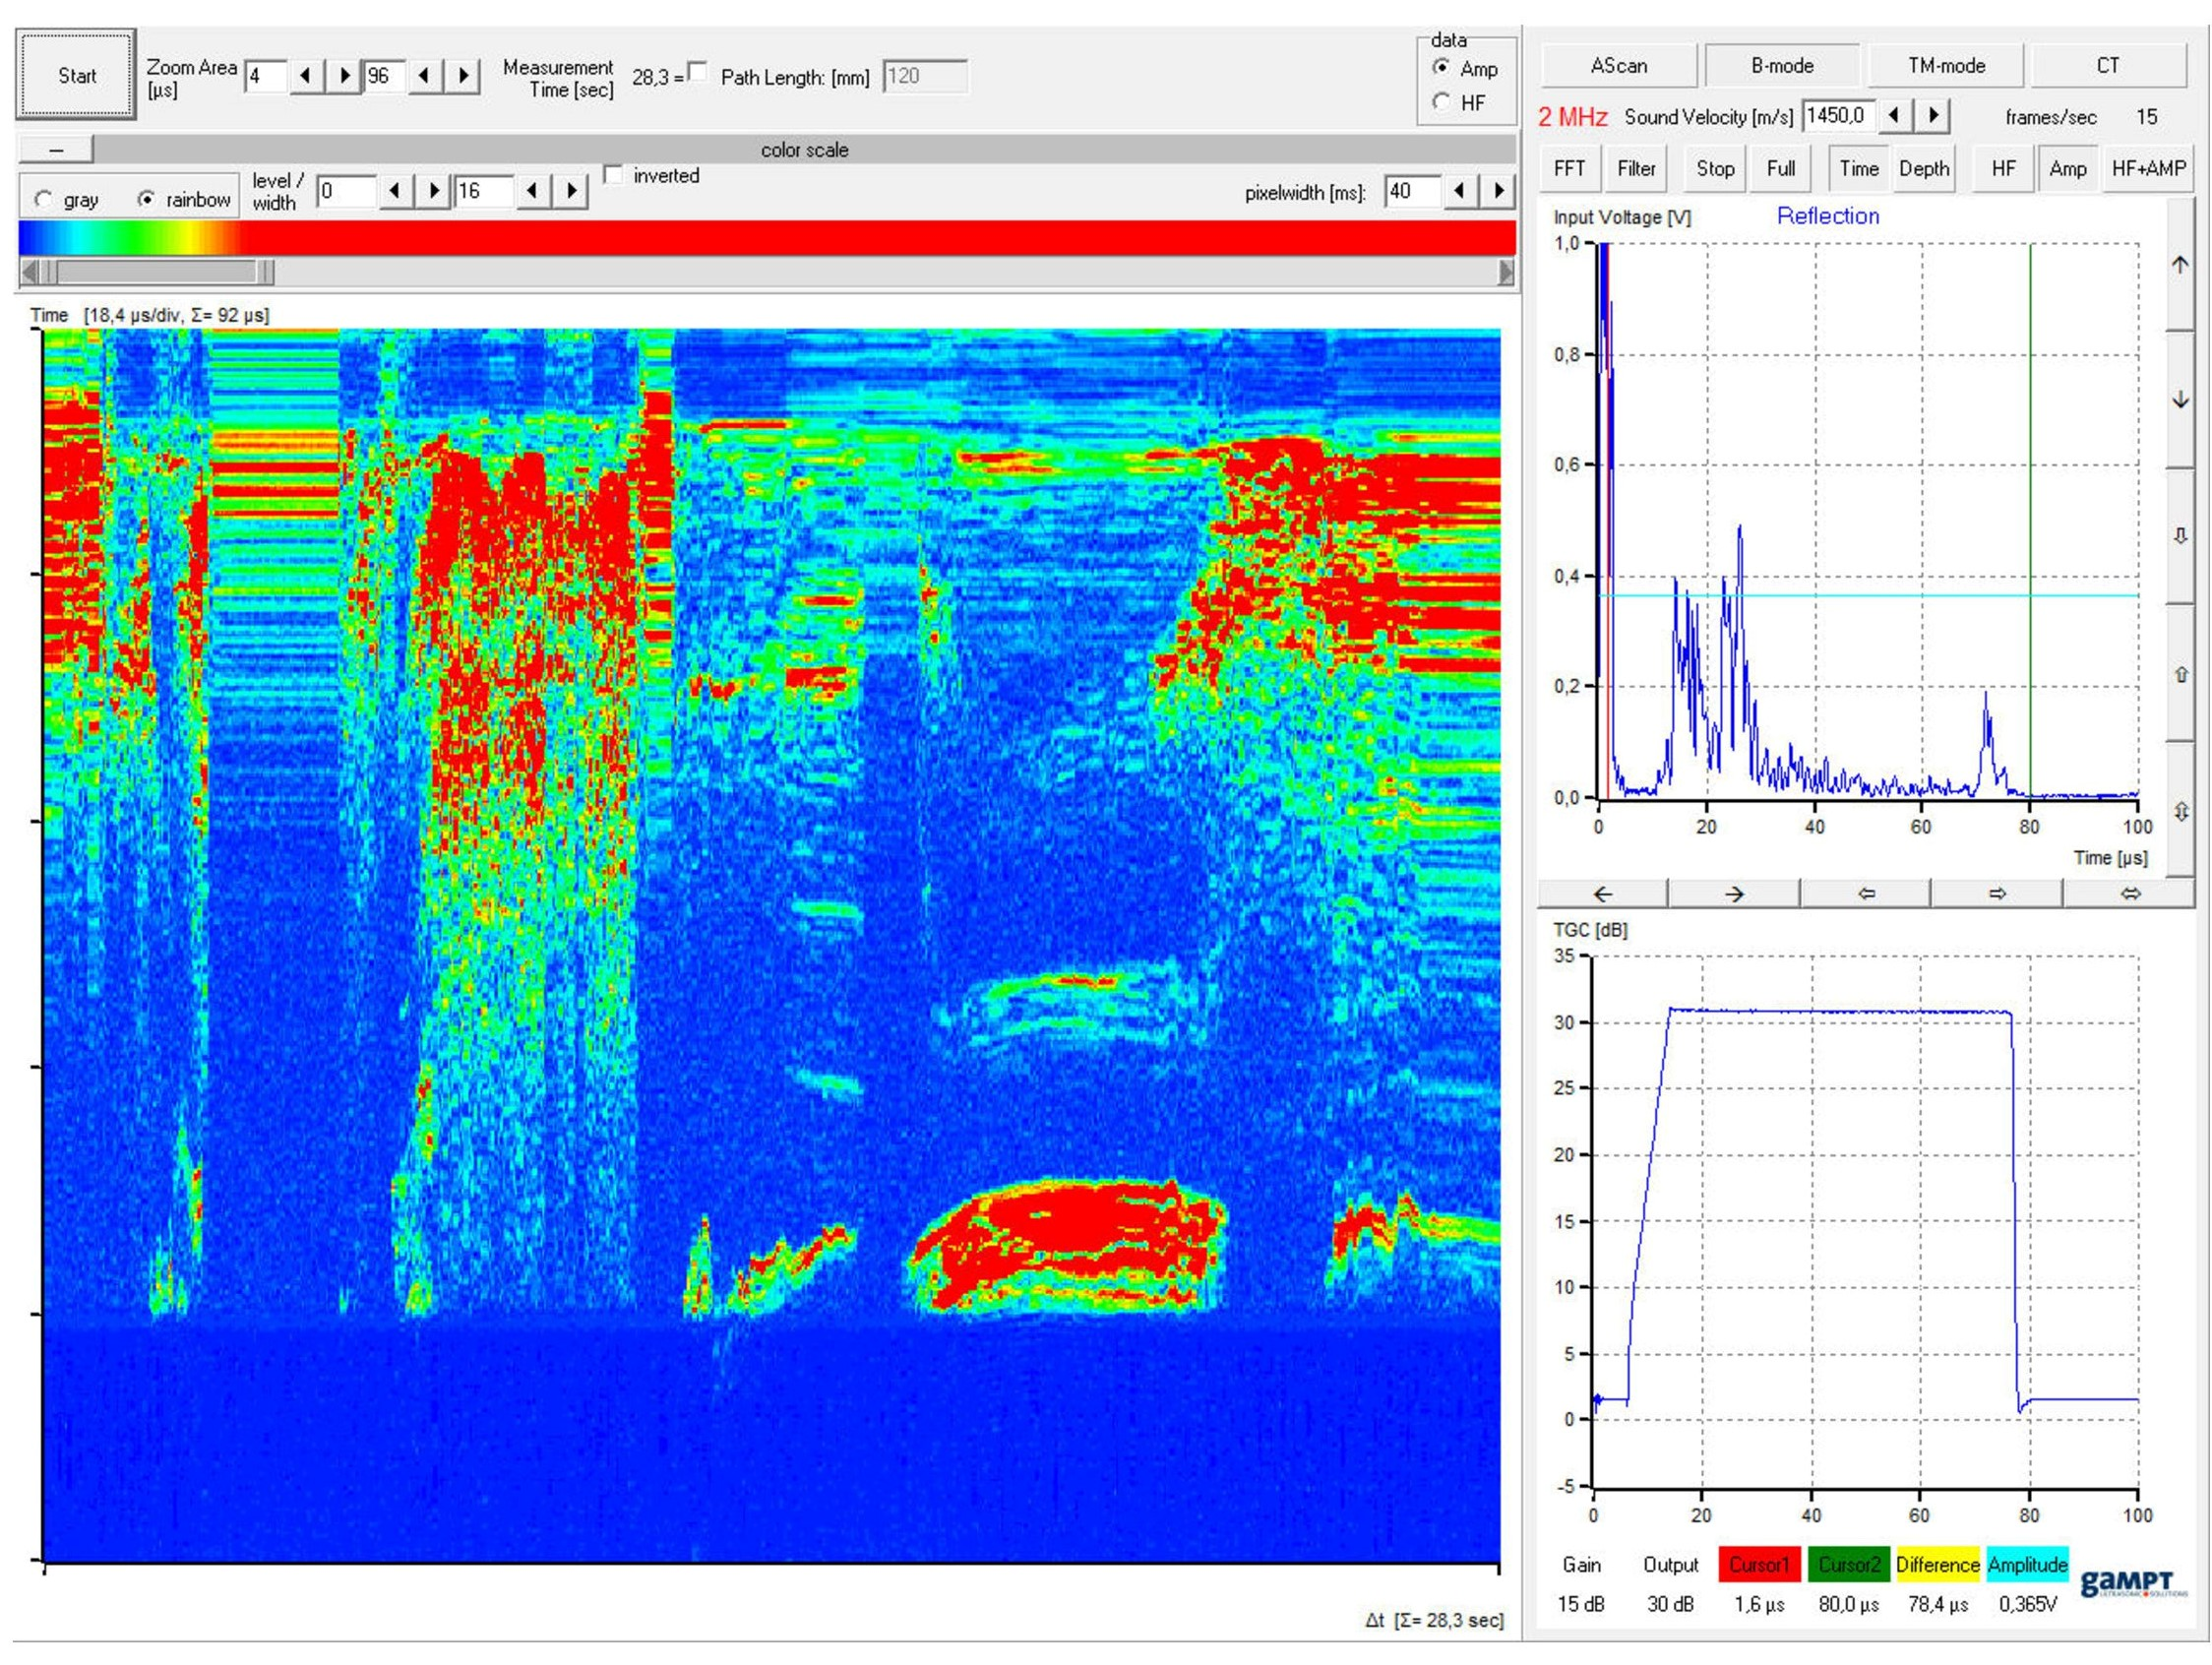
\includegraphics[width=\textwidth]{messwerte/Boobie/Untengross.jpg}
  \caption{B-Scan des größeren Tumors in der unteren Brust.}
  \label{fig:gross}
\end{figure}